%%
%% This is file `sample-acmlarge.tex',
%% generated with the docstrip utility.
%%
%% The original source files were:
%%
%% samples.dtx  (with options: `acmlarge')
%% 
%% IMPORTANT NOTICE:
%% 
%% For the copyright see the source file.
%% 
%% Any modified versions of this file must be renamed
%% with new filenames distinct from sample-acmlarge.tex.
%% 
%% For distribution of the original source see the terms
%% for copying and modification in the file samples.dtx.
%% 
%% This generated file may be distributed as long as the
%% original source files, as listed above, are part of the
%% same distribution. (The sources need not necessarily be
%% in the same archive or directory.)
%%
%% The first command in your LaTeX source must be the \documentclass command.
\documentclass[acmlarge,noacm]{acmart}
\bibliographystyle{unsrt}
\settopmatter{printacmref=false} % Removes citation information below abstract
\renewcommand\footnotetextcopyrightpermission[1]{} % removes footnote with conference information in first column
\pagestyle{plain} % removes running headers

%%
%% \BibTeX command to typeset BibTeX logo in the docs
\AtBeginDocument{%
  \providecommand\BibTeX{{%
    \normalfont B\kern-0.5em{\scshape i\kern-0.25em b}\kern-0.8em\TeX}}}

\usepackage{tabu}                      % only used for the table example
\usepackage{booktabs}                  % only used for the table example
\usepackage{multirow}
\usepackage{tabularx}

%%
%% end of the preamble, start of the body of the document source.
\begin{document}

%%
%% The "title" command has an optional parameter,
%% allowing the author to define a "short title" to be used in page headers.
\title{Clustering algorithms on GPU}
\subtitle{Team 18}
%%
%% The "author" command and its associated commands are used to define
%% the authors and their affiliations.
%% Of note is the shared affiliation of the first two authors, and the
%% "authornote" and "authornotemark" commands
%% used to denote shared contribution to the research.
\author{Deepam Sarmah}
\email{deepam20050@iiitd.ac.in}

\renewcommand{\shortauthors}{Deepam Sarmah}

%%
%% This command processes the author and affiliation and title
%% information and builds the first part of the formatted document.
\maketitle

\section{Introduction}
In the day and age of data science, there has been an increased demand for clustering algorithms. Clustering algorithms cluster similar data points based on their characteristics or features. They are helpful in many cases. To name a few, they help segment the data into meaningful groups based on a standard metric (these can be maximum revenue,  average life expectancy, etc.) and anomaly detection, where clustering algorithms can help identify outliers or anomalies in the data by identifying data points that do not belong to any cluster (this is helpful in cancer detection). GPUs help increase the efficiency of clustering algorithms mainly due to the following: Many clustering algorithms are computationally intensive, and hence the GPU could parallelize these computations. Another benefit is that GPUs provide a larger memory bandwidth and processing power, making GPUs ideal for clustering large data-sets. In this project, I aim to compare the serial and parallel implementations of K-Means, DBSCAN, and Mean-Shift clustering algorithms and compute speedup statistics on the same.


\section{Literature review}
There are several clustering algorithms such as K-Means, DBSCAN and Mean-Shift algorithm. I reviewed their research papers and implementations online.

\subsection{K-Means Algorithm}

The K-Means algorithm was first proposed by MacQueen in 1967 \cite{macqueen1967classification} and then later enhanced by Hartigan and Wong \cite{hartigan1979k} in 1979. The K-Means algorithm is an unsupervised clustering algorithm in which the algorithm starts by randomly selecting a number of data points as the initial centroids for each cluster. Then, each data point in the dataset is assigned to the cluster whose centroid is closest to it. Next, the centroids are recalculated as the mean of all data points in the cluster. This process of assigning points to the closest cluster and recalculating centroids is repeated until a maximum number of iterations is reached. The result is $k$ clusters, each represented by a centroid, where the data points in each cluster are similar to each other and different from those in the other clusters. There have been implementations of K-Means on GPUs using CUDA by Reza Farivar, et al. \cite{farivar2008parallel} in 2008. The K-Means algorithms is useful as it can handle large data-sets and can converge to the solution quickly.  

\subsection{DBSCAN Algorithm}
Density-based spatial clustering of applications with noise (DBSCAN) is a data clustering algorithm proposed by Martin Ester, et al. \cite{10.5555/3001460.3001507} in 1996. A GPU implmentation of DBSCAN was proposed by Guilherme Andrade, et al. \cite{andrade2013g} in 2013. DBSCAN works by defining two important parameters: the radius $\epsilon$ and the minimum number of points required to form a cluster (say $\Phi$). It starts with a random data point, and builds a cluster around it by identifying all points within a distance of  $\epsilon$. If the number of points in this region is greater than or equal to $\Phi$, then a new cluster is formed. Otherwise, the point is marked as noise or an outlier. DBSCAN then continues to grow the cluster by recursively finding new points within the $\epsilon$ radius and adding them to the cluster until no new points can be added. The algorithm repeats this process for all unvisited points in the dataset, assigning them to clusters or marking them as noise. DBSCAN is highly useful as it can handle non-spherical clusters and can identify the number of clusters based on the density of the data.

\subsection{Mean-Shift Algorithm}
A description of the Mean-Shift algorithm is found in the paper by K Fukunaga, et al. \cite{fukunaga1975estimation} in 1975. The mean shift algorithm works by by randomly selecting a data point and defining a window around it. The mean of all data points within the window is then computed, and the window is shifted towards this mean. This process is repeated for each window until the window no longer moves or changes significantly. At the end of the process, each data point is assigned to the nearest converged window, which represents a cluster. The Mean-Shift algorithm is advantageous as it can handle large data-sets with many features and is suitable for clustering data-sets with complex cluster shapes.


\section{Milestones}
The identified milestones are:
\begin{table}[!h]
\label{tbl:milestones}
\begin{center}
\begin{tabu} to \textwidth {rXl} \toprule
\textbf{S. No.} & \textbf{Milestone} & \textbf{Member}\\\midrule
1 & Implement K-Means on CPU & Deepam\\
2 & Implement Mean-Shift on CPU & Deepam \\
3 & Implement K-Means and Mean-Shift on GPU & Deepam\\
4 & Implement DBSCAN on CPU & Deepam \\
5 & Implement DBSCAN on GPU & Deepam \\
6 & Compare and analyze GPU code using profiler & Deepam \\
\bottomrule
\end{tabu}
\end{center}
\end{table}

%\section{Approach}
% Discuss your approach here. (in mid-evaluation submission)
% Include algorithm analysis, challenges and approach.


%\section{Results}
% Discuss results here. (in mid-evaluation submission
% Include output, performance tables and graphs. Comparison with CPU-GPU and with other codes directly related to this work.

% Results may have images.
%\begin{figure}[h]
%  \centering
%  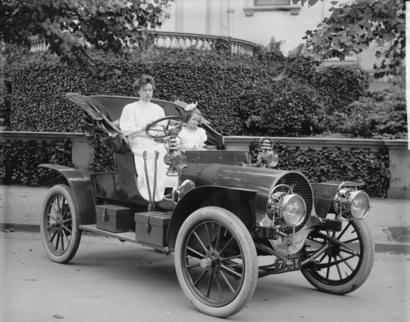
\includegraphics[width=\linewidth]{./images/sample-franklin}
%  \caption{1907 Franklin Model D roadster. Photograph by Harris \&
%    Ewing, Inc. [Public domain], via Wikimedia
%    Commons. (\url{https://goo.gl/VLCRBB}).}
%  \Description{A woman and a girl in white dresses sit in an open car.}
%\end{figure}
%
%Your figures should contain a caption which describes the figure to
%the reader.
%
%Figure captions are placed {\itshape below} the figure.

%\section{Conclusion}
% Conclude here (in final submission)


%%
%% The next two lines define the bibliography style to be used, and
%% the bibliography file.
\bibliographystyle{ACM-Reference-Format}
\bibliography{Report_Project_01_Group_01}

\end{document}